\documentclass[aspectratio=169,11pt,hyperref={colorlinks=true}]{beamer}
% https://github.com/zr-tex8r/BXcjkjatype/blob/master/README-ja.md
\usepackage[whole]{bxcjkjatype}
\usetheme{boxes}
\setbeamertemplate{navigation symbols}{}
\definecolor{suse}{RGB}{2, 211, 95}
\definecolor{susedark}{RGB}{13, 44, 64}
\definecolor{linkcolor}{RGB}{13, 44, 255}
\setbeamercolor{titlelike}{fg=suse}
\setbeamercolor{structure}{fg=suse}
\hypersetup{colorlinks,urlcolor=suse}
\setbeamertemplate{footline}[frame number]
% Inserting graphics
\usepackage{graphicx}
% Side-by-side figures, etc
\usepackage{subfigure}
% Code snippits
\usepackage{listings}
% Color stuff
\usepackage{color}
% underline
\usepackage{soul}
% calc
\usepackage{calc}

\usepackage{amsmath}
\usepackage{tikz}
\newcommand\RBox[1]{%
  \tikz\node[draw,rounded corners,align=center,] {#1};%
}
\usepackage{hyperref}
%\usecolortheme{buzz}
%\usecolortheme{wolverine}
%\usetheme{Boadilla}
\usepackage[T1]{fontenc}
%\usepackage{fontspec}
%\usepackage[expert, deluxe]{otf}

\definecolor{mygreen}{rgb}{0,0.6,0}
\definecolor{mygray}{rgb}{0.5,0.5,0.5}
\definecolor{mymauve}{rgb}{0.58,0,0.82}


%\usepackage{CJK}
%\pdfmapline{=genshingothic@Unicode@ <genshingothic.ttf}
% bxcjkjatype
%\setgothicfont[<ID>]{<フォントファイル名>}
%\setgothicfont{/Users/foo/Library/Fonts/genshingothic.ttf}
%\setgothicfont{/Users/foo/Library/Fonts/NotoSansCJKjp-Regular.otf}
%\setgothicfont{/Users/foo/Downloads/genshingothic-20150607/GenShinGothic-P-Normal.ttf}
%\setgothicfont{/Users/foo/Downloads/genshingothic-20150607/GenShinGothic-Regular.ttf}
%\setgothicfont{hiragino.ttc}
\setgothicfont{mplus-1p-regular.ttf}
\setCJKfamilydefault{\gtdefault}
%\setCJKfamilydefault{\mcdefault}
%\CJKforce{abcdefghijklmnopqrstuvwxyzABCDEFGHIJKLMNOPQRSTUVWXYZ}


\lstset{%
  backgroundcolor=\color{susedark},   % choose the background color; you must add \usepackage{color} or \usepackage{xcolor}
  breakatwhitespace=false,         % sets if automatic breaks should only happen at whitespace
  breaklines=true,                 % sets automatic line breaking
  captionpos=b,                    % sets the caption-position to bottom
  commentstyle=\color{suse},  % comment style
  extendedchars=true,              % lets you use non-ASCII characters; for 8-bits encodings only, does not work with UTF-8
  keepspaces=true,                 % keeps spaces in text, useful for keeping indentation of code (possibly needs columns=flexible)
  keywordstyle=\color{blue},       % keyword style
%  otherkeywords={*,...},           % if you want to add more keywords to the set
  numbersep=5pt,                   % how far the line-numbers are from the code
  numberstyle=\tiny\color{mygray}, % the style that is used for the line-numbers
  rulecolor=\color{white},         % if not set, the frame-color may be changed on line-breaks within not-black text (e.g. comments (green here))
  showspaces=false,                % show spaces everywhere adding particular underscores; it overrides 'showstringspaces'
  showstringspaces=false,          % underline spaces within strings only
  showtabs=false,                  % show tabs within strings adding particular underscores
  stringstyle=\color{suse},   % string literal style
}

\setbeamerfont{caption}{series=\normalfont,size=\fontsize{6}{8}}
%\setbeamerfont{caption}{series=\normalfont,size=\large}
\setbeamertemplate{caption}{\raggedright\insertcaption\par}

\setlength{\abovecaptionskip}{0pt}
\setlength{\floatsep}{0pt}

%%%%%%%%%%%%%%%%%%%%%%%%%%%%%%%%%%%%%%%%%%%%%%%%%%%%%%%%%%%%%%%%%%%%%

\author[Masayuki Igawa]{%
    \texorpdfstring{%
            \centering
            Masayuki Igawa\\
            \href{mailto:masayuki@igawa.io}{masayuki@igawa.io}\\
            \texttt{masayukig on
              \href{https://freenode.net/}{Freenode},
              \href{https://github.com/masayukig}{GitHub},
              \href{https://twitter.com/masayukig}{Twitter},
              \href{https://www.linkedin.com/in/masayukig/}{LinkedIn}}
    }
    {Masayuki Igawa}
}
\date{\href{https://2019.fossasia.org/event/schedule.html}{March 15, 2019}}
\def\place#1{\def\@place{#1}}
\place{\href{https://2019.fossasia.org/event/schedule.html\#5131}{@FOSSASIA Summit 2019}}

%\vspace*{10pt}
\title[k8s-the-hard-way
  \hspace{4em}\insertframenumber/\inserttotalframenumber]{\Huge{Kubernetes The Hard Way}}

\setbeamercolor{background canvas}{bg=susedark}
\setbeamercolor{titlelike}{fg=white}
\setbeamercolor{structure}{fg=white}
\setbeamercolor{normal text}{fg=white}

\begin{document}
%\setbeamertemplate{background canvas}{
\includegraphics[width=\paperwidth,height=\paperheight]{images/opensuse_base.png}}
{%
% \setbeamertemplate{background canvas}{
\includegraphics[width=\paperwidth,height=\paperheight]{images/opensuse_preface.png}}
\setbeamertemplate{footline}{}
\setbeamercolor{background canvas}{bg=susedark}
\begin{frame}[noframenumbering]
  \hypersetup{colorlinks,urlcolor=suse}
  \setbeamercolor{author}{fg=white}
  \setbeamercolor{date}{fg=white}
  \setbeamercolor{place}{fg=white}
  \titlepage{}
  \centering
  \@place \par
  \href{https://bit.ly/k8s-the-hard-way-fossasia2019}{https://bit.ly/k8s-the-hard-way-fossasia2019}
  \begin{flushright}
    \tiny\href{https://creativecommons.org/licenses/by/4.0/}{This work
      is licensed under a Creative Commons Attribution 4.0
      International License unless.}~
\includegraphics[scale=0.3]{images/cc_by.png}
  \end{flushright}
\end{frame}
}

\section{Agenda}
\begin{frame}
  \frametitle{Agenda}
  \begin{enumerate}
    \item Who am I?
    \item Today's Goal
    \item What's ``Kubernetes The Hard Way''?
    \item Kubernetes The Hard Way on GCP
    \item Kubernetes The Hard Way on OpenStack
    \item Conclusion
%    \item Demo
  \end{enumerate}
\end{frame}

\section{DISCLAIMER}
\begin{frame}
  \frametitle{DISCLAIMER}
  \Huge{\bf{These slides are my own opinion}}
\end{frame}

\section{Who I am?}
\begin{frame}
  \frametitle{Who I am?}
  \begin{itemize}
    \item Company:1998.4-2015.12 Traditional IT company in Japan,
      2016.1-2017.3 HPE -> 2017.3- SUSE/Novell Japan -> 2019(\href{https://www.suse.com/c/further-independence-for-suse/}{\scriptsize{``Further Independence for SUSE''}})
      \begin{itemize}
        \item SUSE OpenStack Cloud QE(Quality Engineering) Team
      \end{itemize}
    \item Job: Senior Software Engineer/Open Source Programmer
      \begin{itemize}
        \begin{scriptsize}
        \item \href{https://www.openstack.org/}{OpenStack}
          \href{https://wiki.openstack.org/wiki/QA}{QA} Up/Downstream development, Core Reviewer
        \item[]
          (\href{https://docs.openstack.org/developer/tempest/}{Tempest},
          \href{http://status.openstack.org/openstack-health/}{OpenStack-Health},
          \href{https://docs.openstack.org/developer/subunit2sql/}{Subunit2SQL},
          \href{https://docs.openstack.org/developer/stackviz/}{Stackviz}),
          \href{https://github.com/mtreinish/stestr}{stestr}
        \item
          \href{http://stackalytics.com/?user_id=igawa&release=all&metric=all}{stackalytics.com/?user\_id=igawa},
          \href{https://github.com/masayukig}{github.com/masayukig}
        \end{scriptsize}
      \end{itemize}
    \item Books 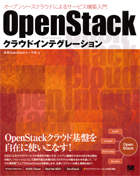
\includegraphics[scale=0.2]{images/OpenStack_Integration_book.png}~
\includegraphics[scale=0.2]{images/InfraCI_book.png}
      \begin{itemize}
      \item \href{https://www.amazon.co.jp/dp/4798139785/}{\scriptsize{OpenStack
        Cloud Integration (Japanese book)}} (one of the authors)
      \item \href{https://www.amazon.co.jp/dp/4798155128/}{\scriptsize{Infra CI
        Pragmatic Guide - Ansible/GitLab (Japanese book)}} (as a reviewer)
      \end{itemize}
    \item Hobby: Bike(BMC SLR02), Clouds(OpenStack...), Diet(Low-carb), etc.
  \end{itemize}
  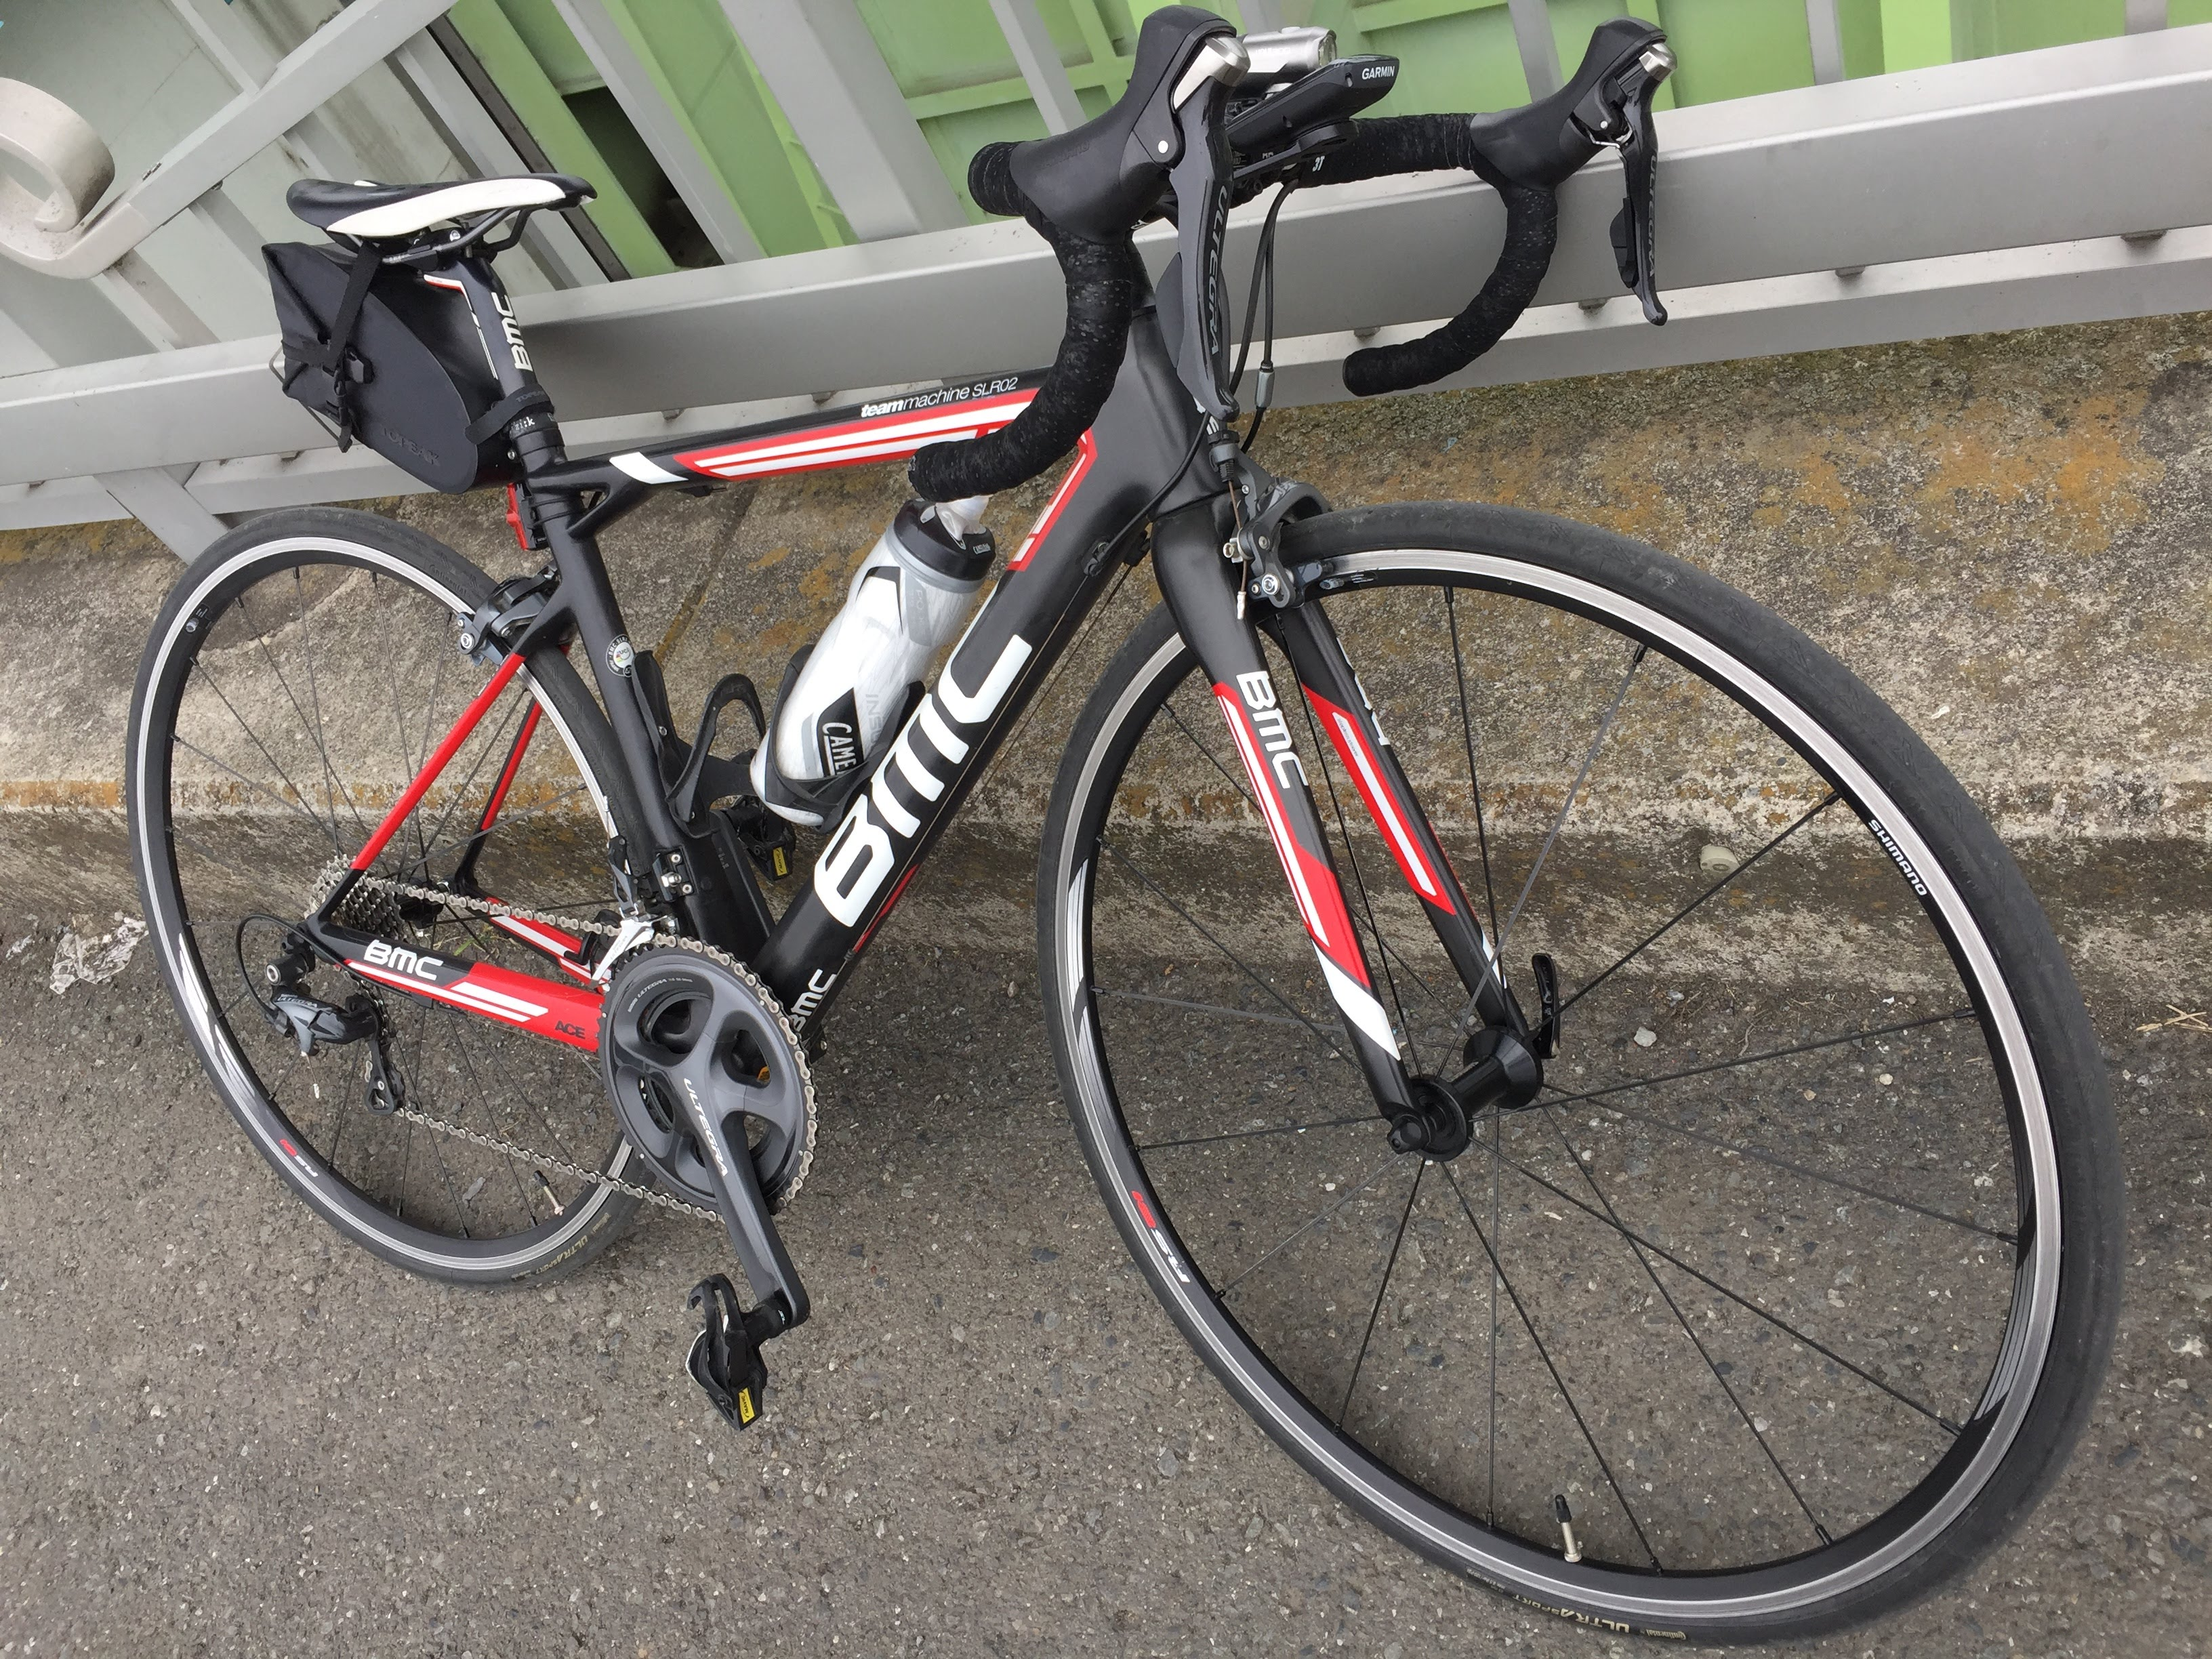
\includegraphics[height=20mm]{images/my-bike.jpg}~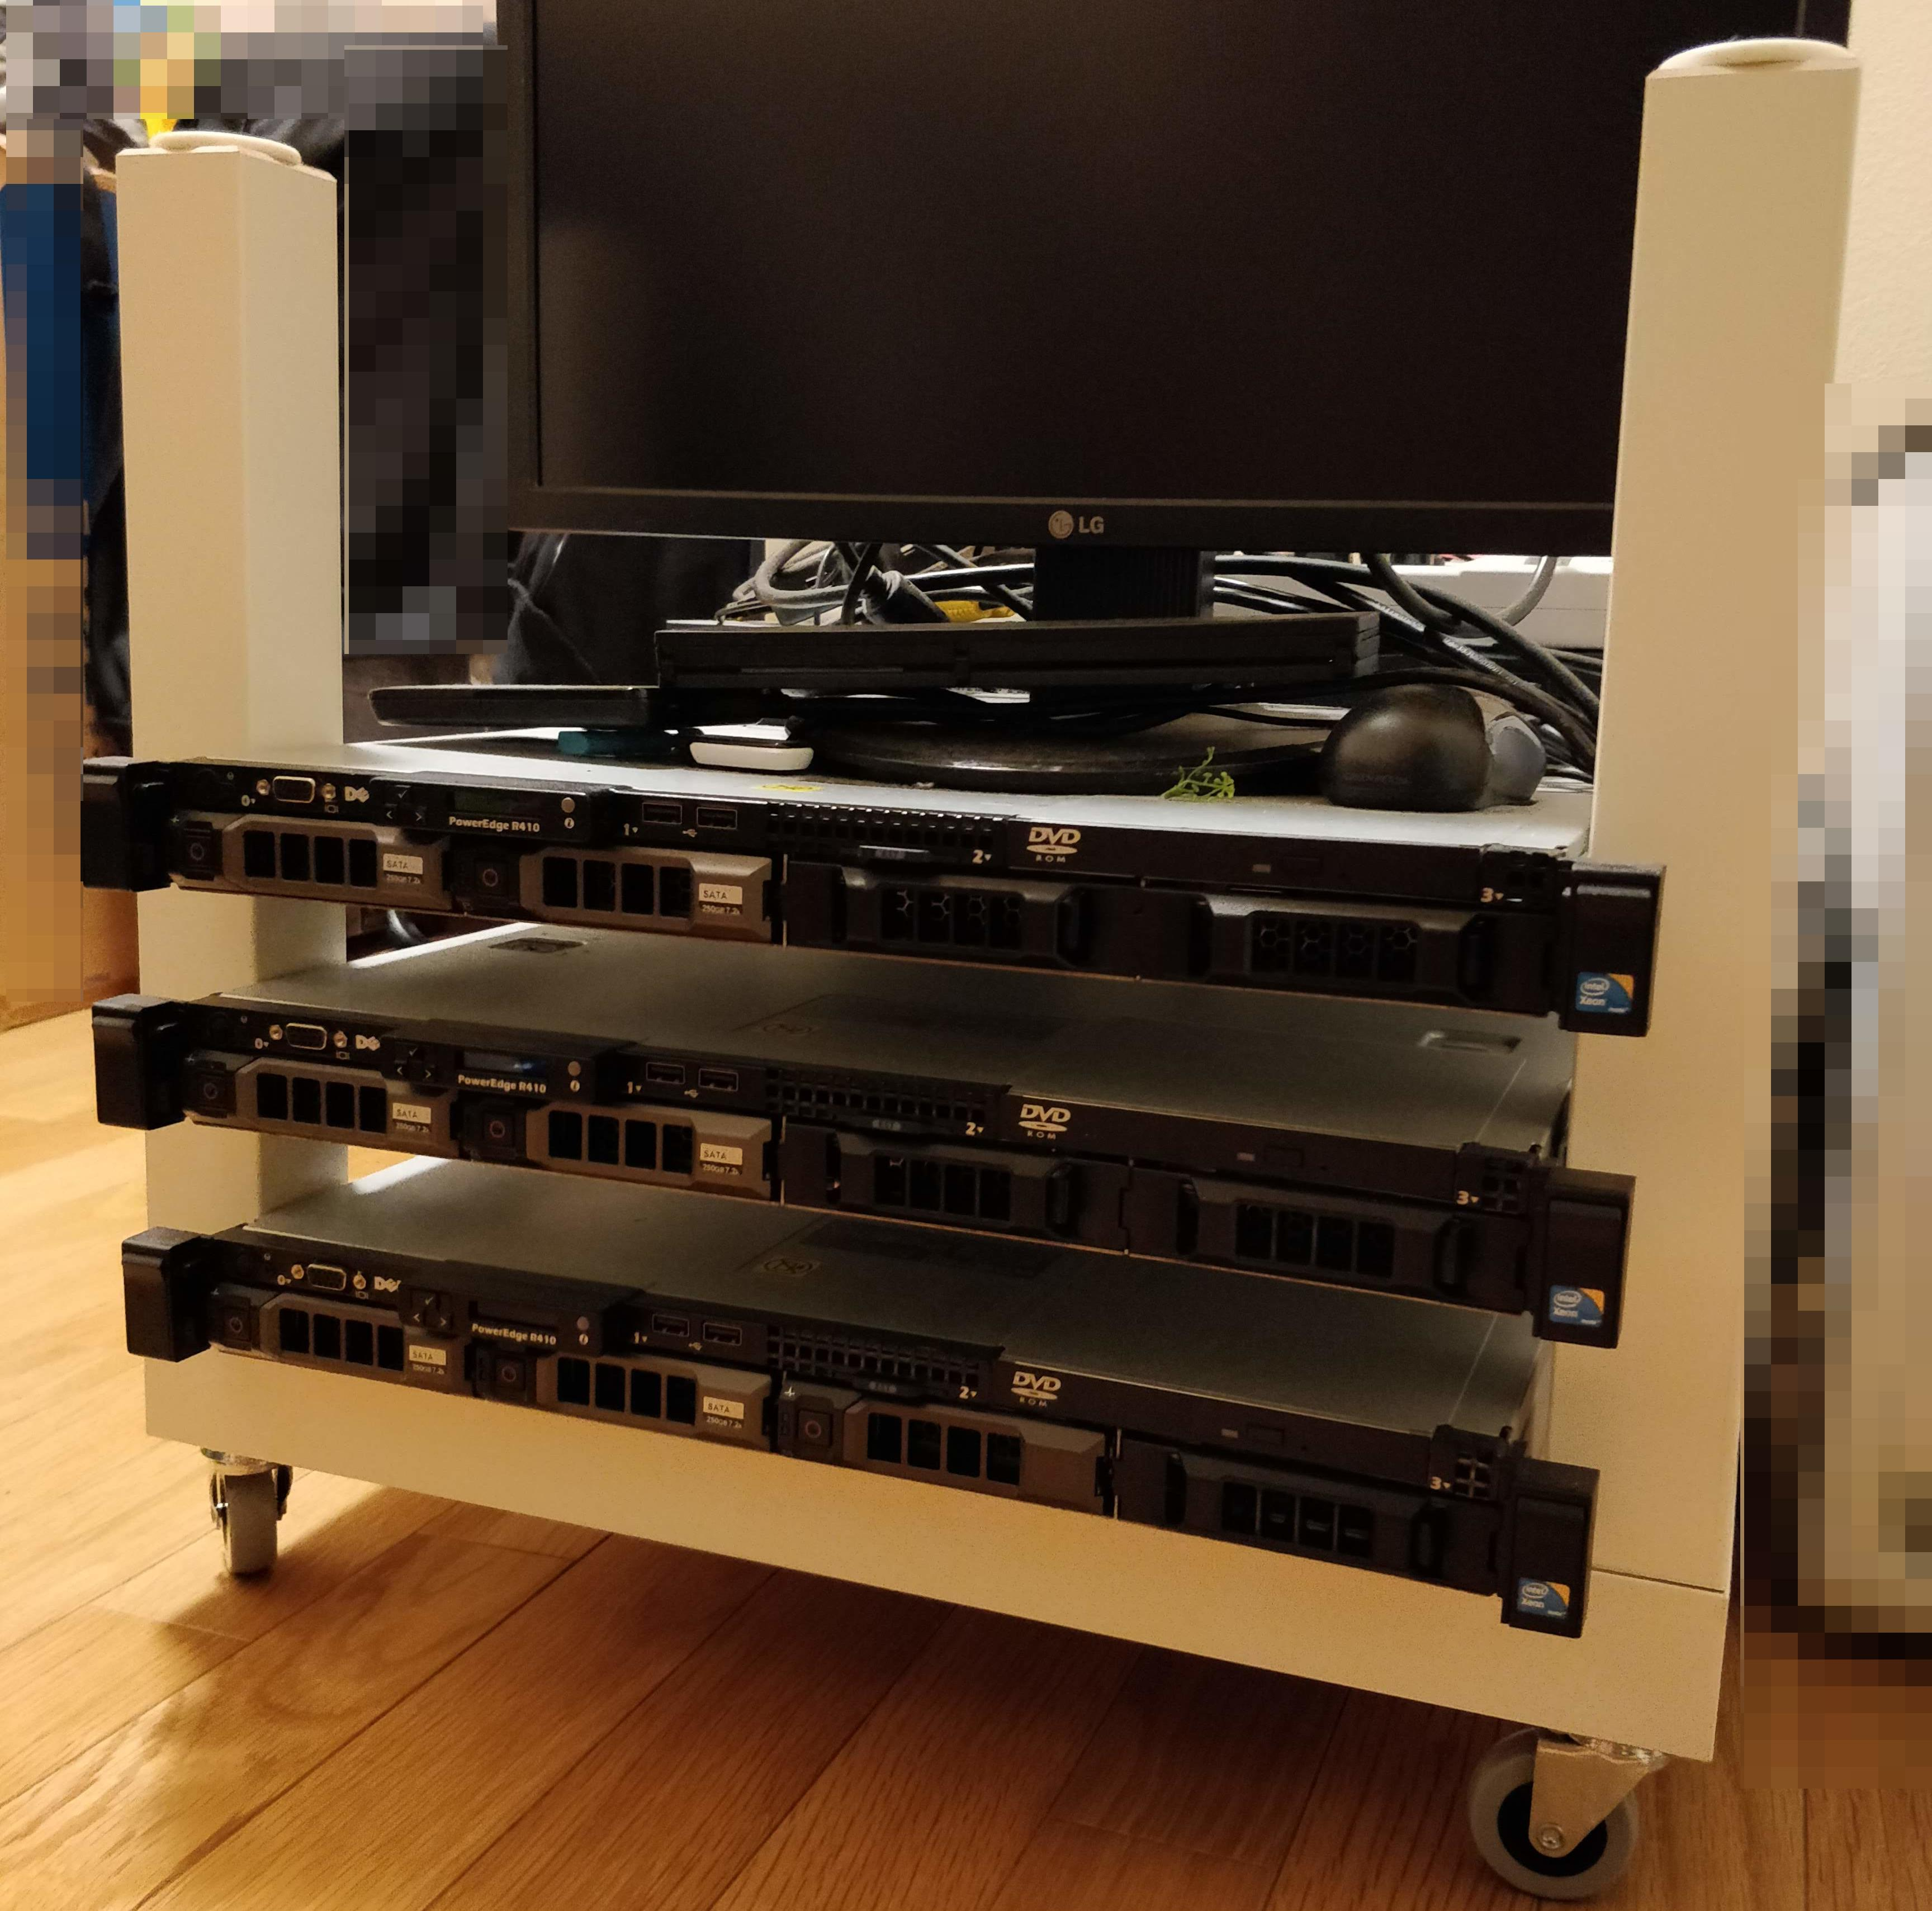
\includegraphics[height=20mm]{images/server_front.jpg}~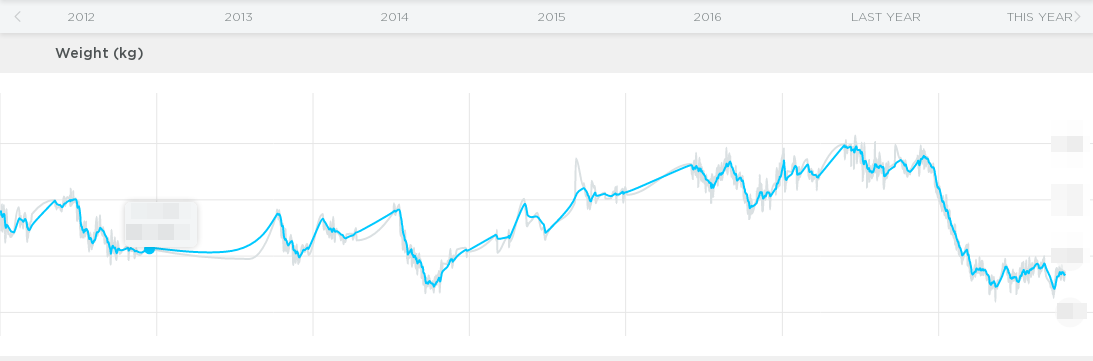
\includegraphics[height=20mm]{images/my-weight.png}
\end{frame}

\section{Goal of today}
\begin{frame}
  \frametitle{Today's Goal}
  \begin{itemize}
    \item Understand ``Kubernetes The Hard Way''
    \item Motivate to do ``Kubernetes The Hard Way'' by yourself
  \end{itemize}
\end{frame}

\section{Introduction}
\begin{frame}
  \frametitle{Do you feel about Kubernetes,}
  \begin{itemize}
    \item[] \Huge{_人人人人人人人人人人人人_}
    \item[] \Huge{>   I have no idea!!   <}
    \item[] \Huge{>   what's going on!? <}
    \item[] \Huge{ ̄YYYYYYYYYYYY ̄}
  \end{itemize}
  When you make a k8s cluster by using minikube, kubeadm, Rancher, GKE/AKS/EKS, etc...
\end{frame}

\begin{frame}
  \frametitle{If you want to...}
  \begin{itemize}
    \item Know its components and architecture
    \item Debug it
    \item Build a k8s cluster as you like
    \item Feel that it's too easy to build a k8s cluster
    \item Understand Kubernetes in detail
    \item Build a k8s cluster in a harder way :-p
  \end{itemize}
  when you make a k8s cluster by using minikube, kubeadm, Rancher, GKE/AKS/EKS, etc...
\end{frame}

\begin{frame}
  \frametitle{If you're interested in one or more, there's}
  \begin{itemize}
    \item[] \Huge{\bf ``Kubernetes the Hard Way''}\large{}
    \item \url{https://github.com/kelseyhightower/kubernetes-the-hard-way}
    \item[] 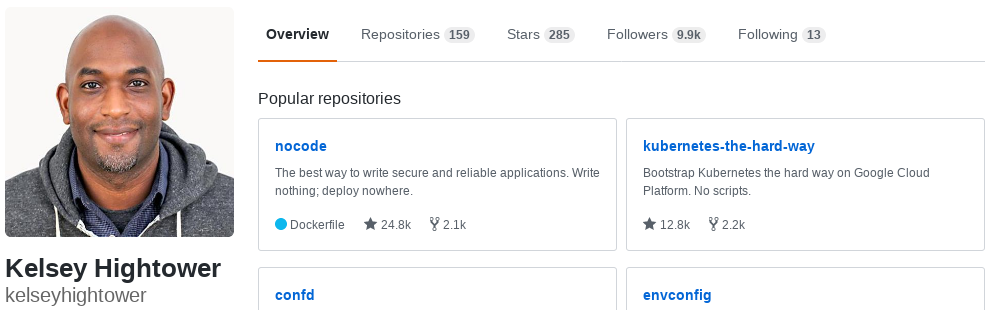
\includegraphics[height=40mm]{images/kelseyhightower_overview.png}
  \end{itemize}
\end{frame}

\section{What is k8s the hard way?}
\begin{frame}
  \frametitle{``Kubernetes the Hard Way'' ?}
  Bootstrap Kubernetes the hard way on GCP. No scripts.
  \begin{itemize}
    \item Tutorial for Kubernetes
    \item Apache License Version 2.0
    \item Document consists of 14 chapters
  \end{itemize}
\end{frame}

\begin{frame}
  \frametitle{``Kubernetes the Hard Way'' ? - components \& versions}
  \begin{itemize}
    \item \href{https://github.com/kubernetes/kubernetes}{Kubernetes} 1.12.0 (Latest: v1.13)
    \item \href{https://github.com/containerd/containerd}{containerd Container Runtime} 1.2.0-rc.0
    \item \href{https://github.com/google/gvisor}{gVisor} 50c283b9f56bb7200938d9e207355f05f79f0d17
    \item \href{https://github.com/containernetworking/cni}{CNI Container Networking} 0.6.0
    \item \href{https://github.com/etcd-io/etcd}{etcd} v3.3.9
    \item \href{https://github.com/coredns/coredns}{CoreDNS} v1.2.2

  \end{itemize}
\end{frame}


\section{What is k8s the hard way?}
\begin{frame}
  \frametitle{``Kubernetes the Hard Way'' ? - outline}
  \begin{enumerate}
    \item Prerequisites
    \item Installing the Client Tools
    \item Provisioning Compute Resources
    \item Provisioning a CA and Generating TLS Certificates
    \item Generating Kubernetes Configuration Files for Authentication
    \item Generating the Data Encryption Config and Key
    \item Bootstrapping the etcd Cluster
    \item Bootstrapping the Kubernetes Control Plane
    \item Bootstrapping the Kubernetes Worker Nodes
    \item Configuring kubectl for Remote Access
    \item Provisioning Pod Network Routes
    \item Deploying the DNS Cluster Add-on
    \item Smoke Test
    \item Cleaning Up
  \end{enumerate}
\end{frame}

\section{What is k8s the hard way?}
\begin{frame}
  \frametitle{``Kubernetes the Hard Way'' ? (partial)}
  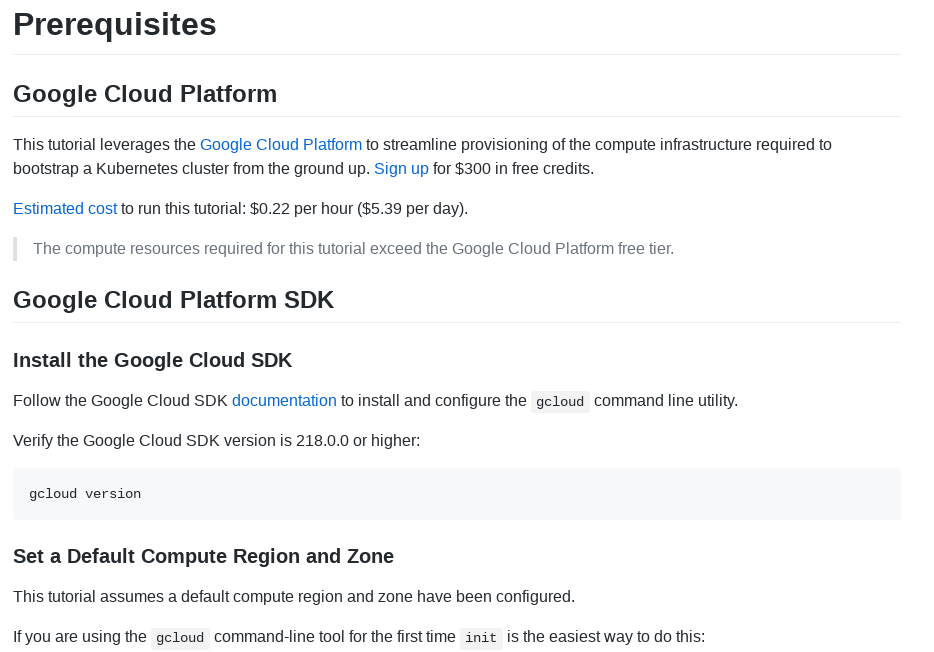
\includegraphics[height=75mm]{images/screenshot-k8s-the-hard-way.png}
\end{frame}

\begin{frame}
  \frametitle{Prerequisites}
  \begin{itemize}
    \item It works on Google Cloud Platform basically.
    \item[] But I could run it on an OpenStack cloud with some tricks :)
    \item n1-standard-1(vCPU*1,MEM: 3.75GB) * 6
    \item[] -> Controller * 3 + Worker * 3 + Load Balancer
  \end{itemize}
\end{frame}

\begin{frame}
  \frametitle{Architechture, components for this k8s cluster}
  \centering{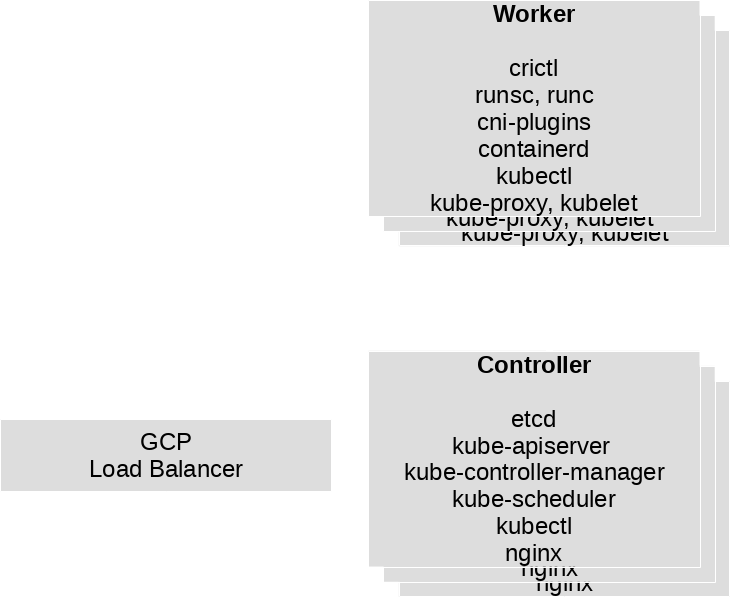
\includegraphics[height=75mm]{images/architecture.png}}
\end{frame}

\section{Conclusion}
\begin{frame}
  \frametitle{Conclusion on GCP}
  \begin{itemize}
    \item Hours: 2.5H, Cost: less than \$1
    \item It says ``Hard way'', but it was not so hard itself.
    \item[]  -> It took only less than 2.5H
    \item I saw some warnings, but you don't need to worry about that that much :)
  \end{itemize}
\end{frame}

\begin{frame}
  \frametitle{Kubernetes The Hard Way on OpenStack Cloud}
  \begin{itemize}
    \item Hardware: \href{https://www.asrock.com/nettop/Intel/DeskMini 310 Series}{ASRock DeskMini 310}, Celeron G4920 3.2GHz, 16GB, 120GB SSD/HDD
    \item Software
      \begin{itemize}
        \item {OS: openSUSE 15, OpenStack version: Rocky, Components: [Nova, Glance, Cinder, Keystone, Neutron]}
        \item Follow the \href{https://docs.openstack.org/install-guide/}{OpenStack Installation Guide} and autemated by ansible
      \end{itemize}
    \item Cost: \$300/node(roughly) * 3
  \end{itemize}
  \begin{figure}
    \begin{tabular}{cc}
      \begin{minipage}[t]{0.45\hsize}
        \centering
        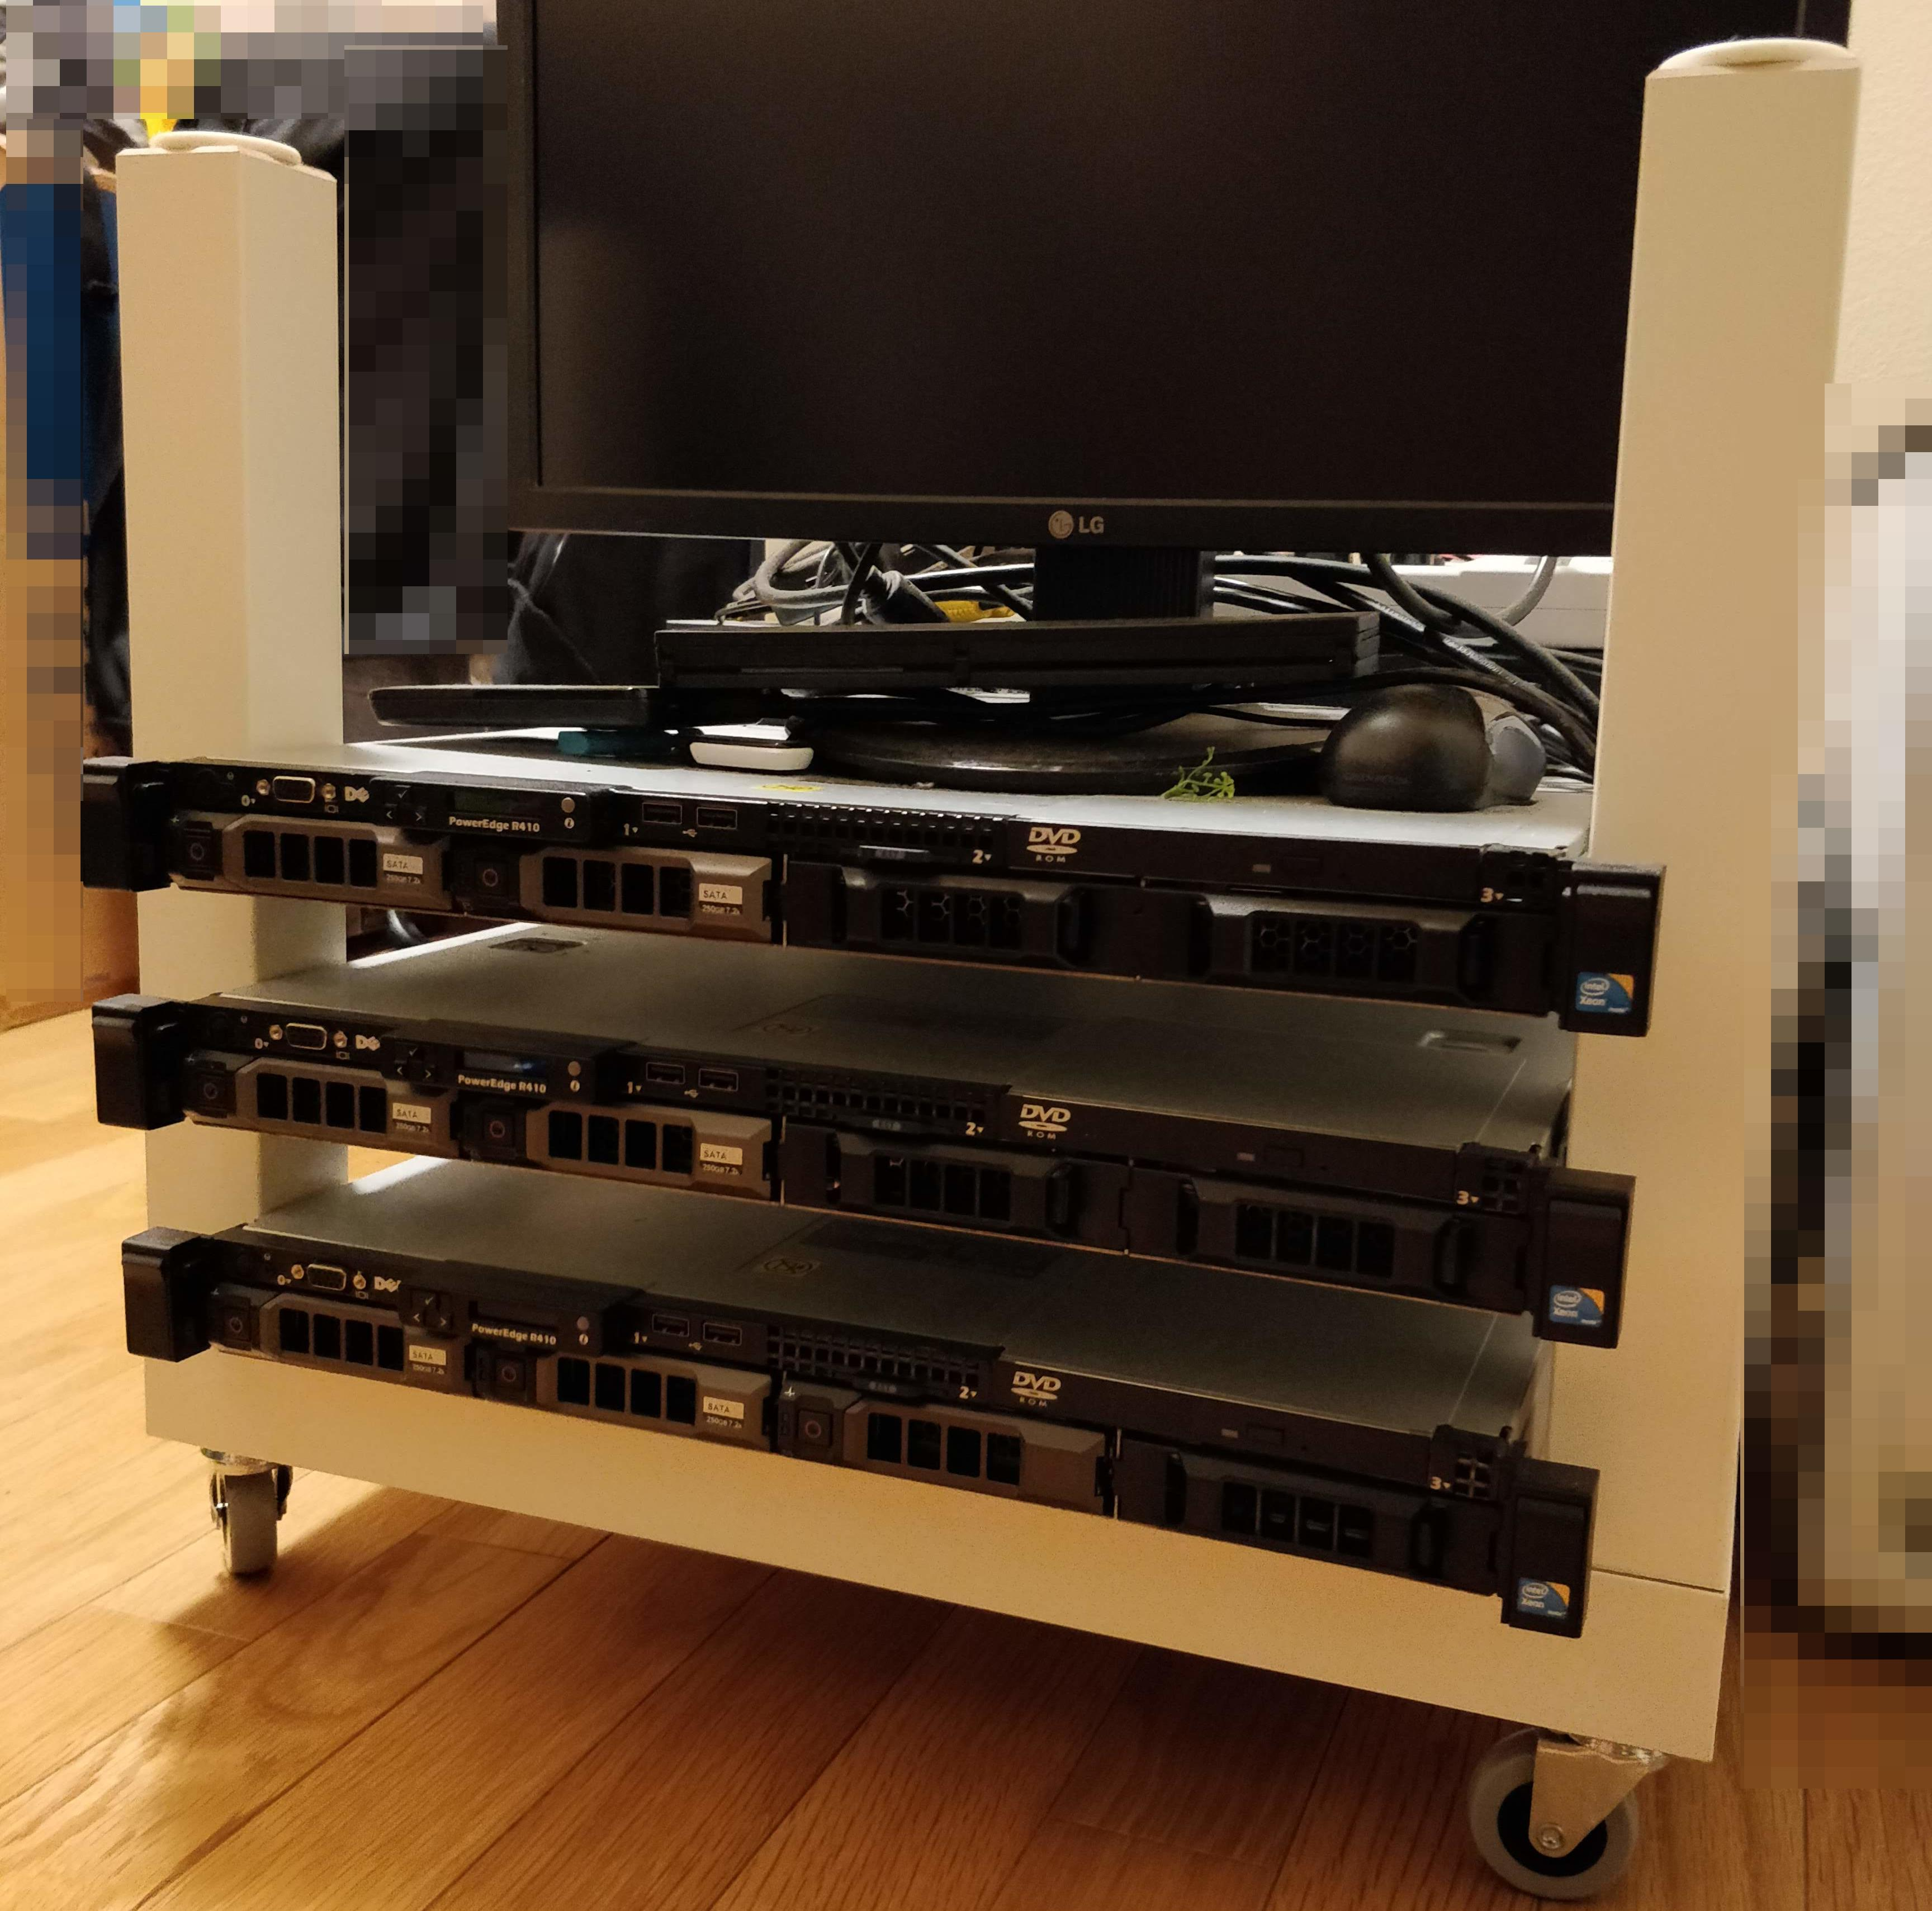
\includegraphics[height=40mm]{images/server_front.jpg}
        \caption{OLD}
      \end{minipage}
      \begin{minipage}[t]{0.45\hsize}
        \centering
        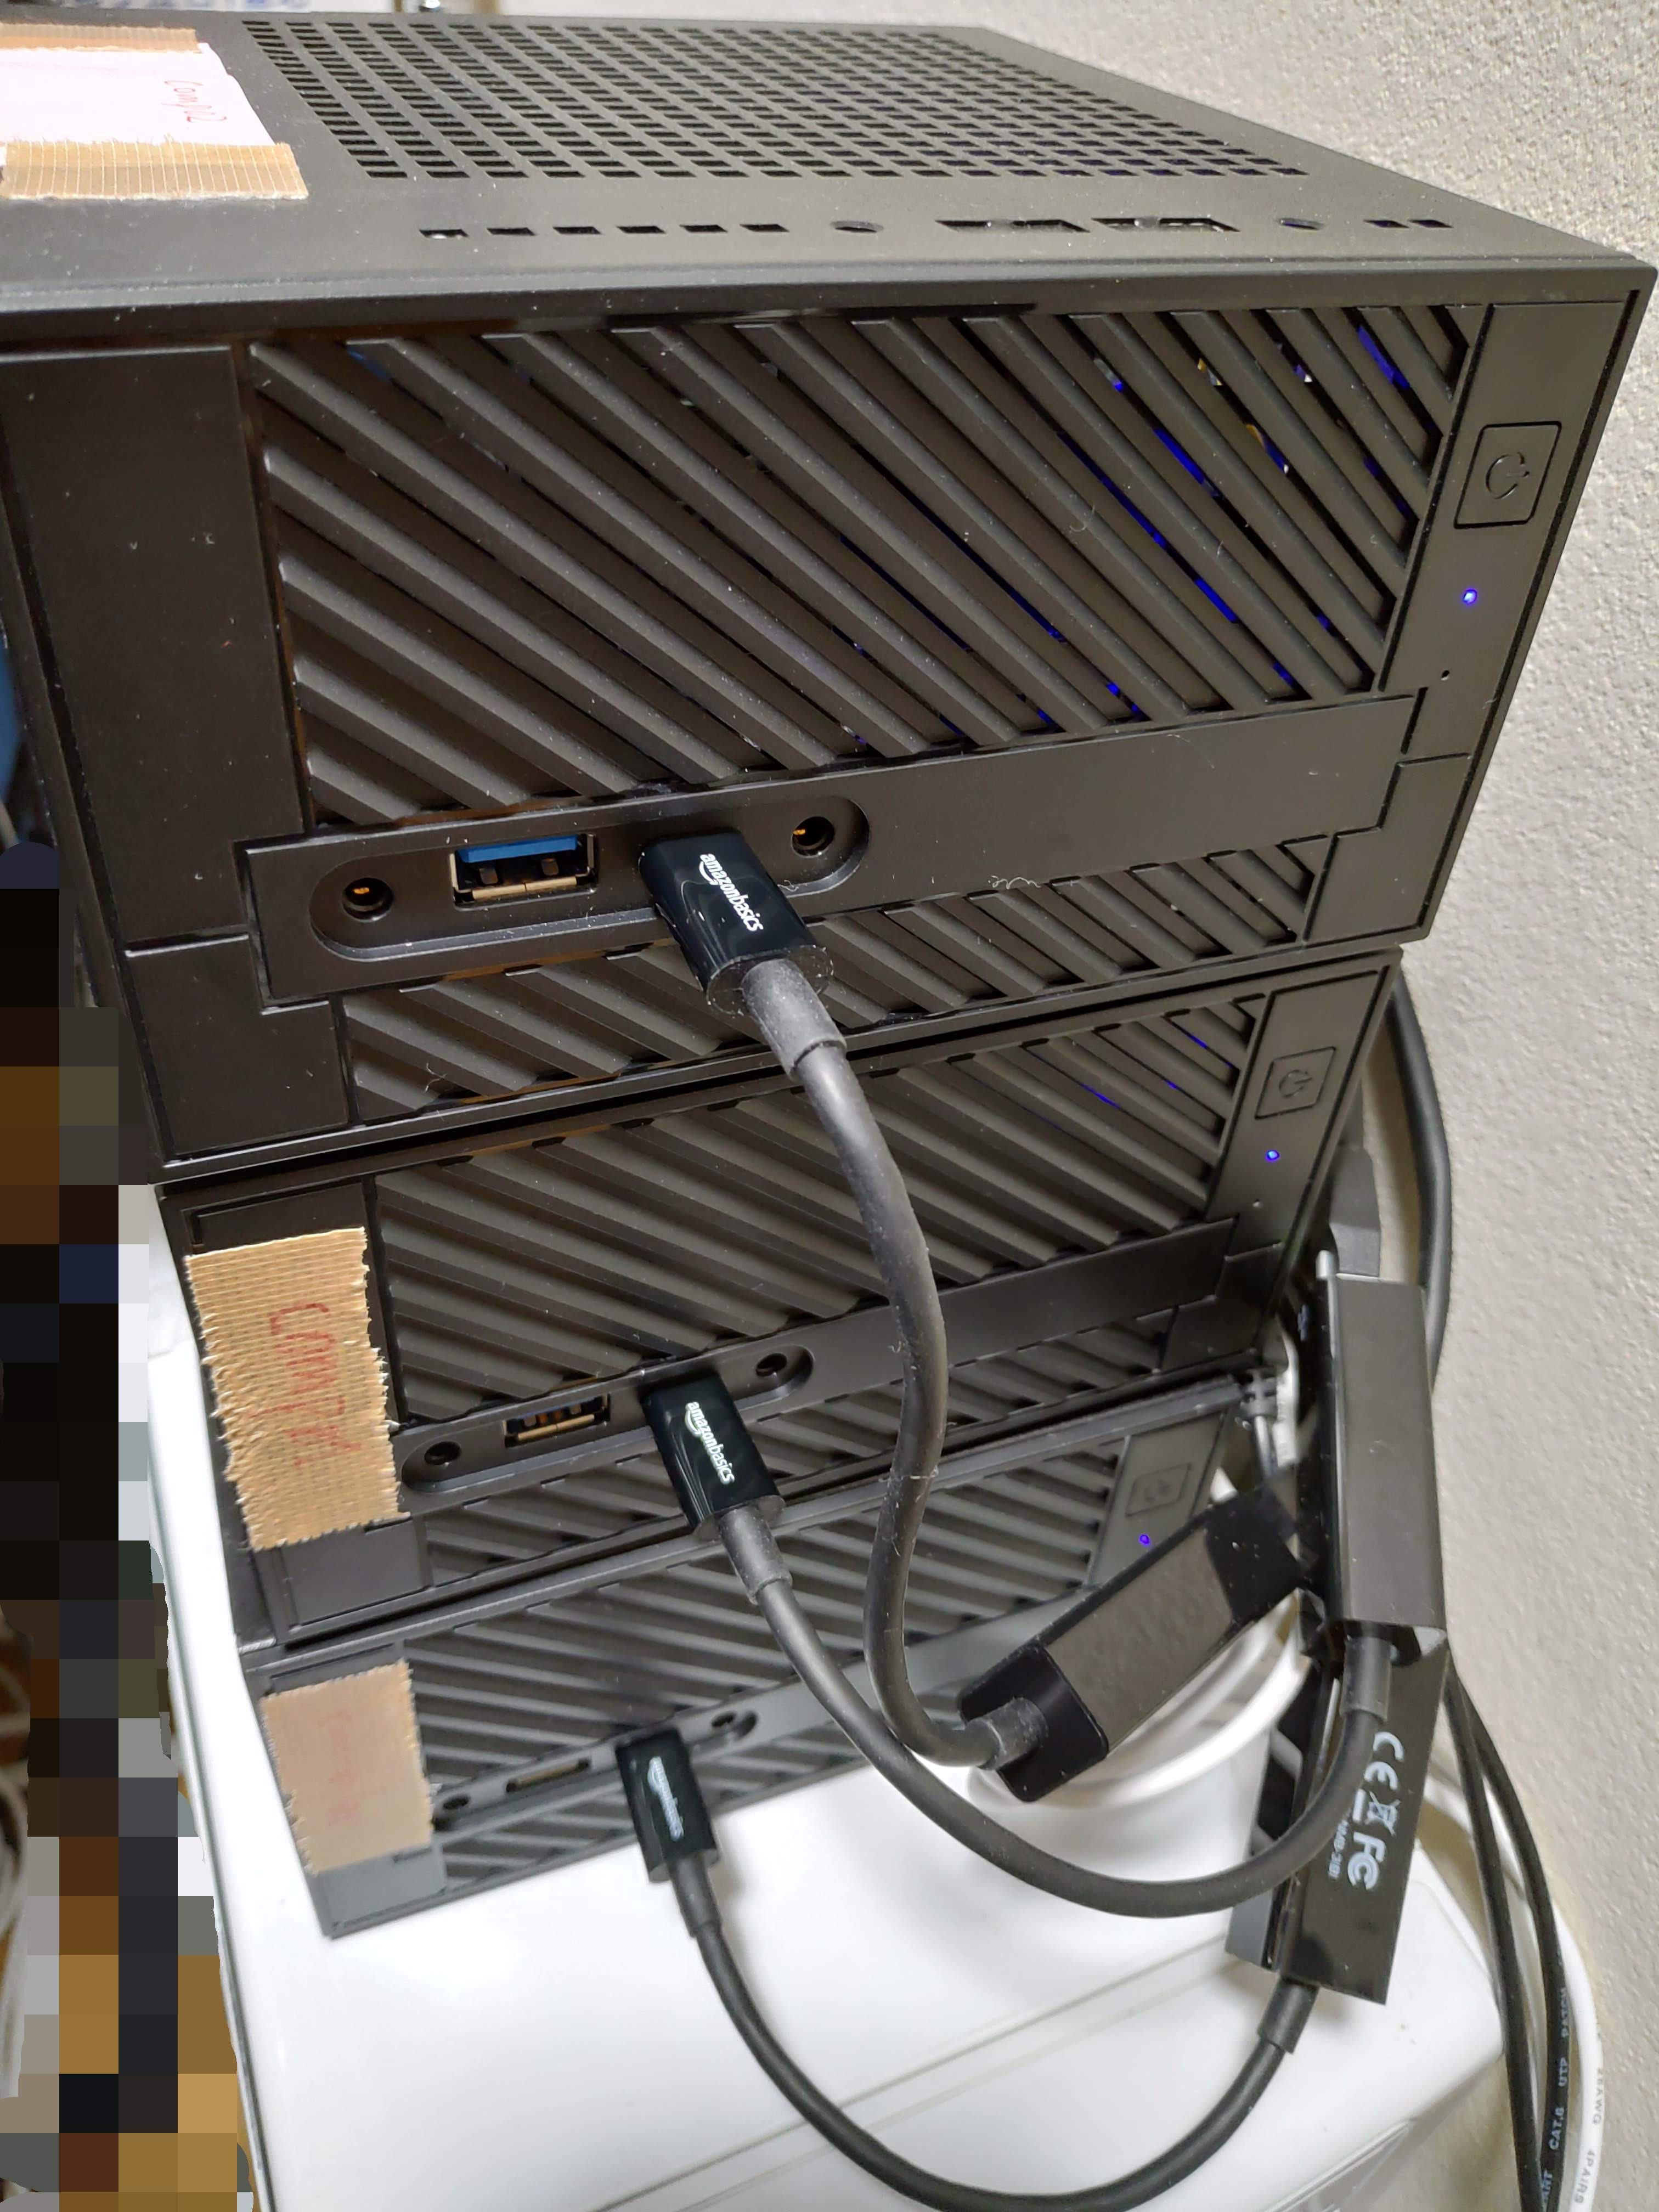
\includegraphics[height=40mm]{images/my-new-cloud.jpg}
        \caption{NEW(smaller, quiet, low energy \& performance)}
      \end{minipage}
    \end{tabular}
  \end{figure}
\end{frame}

\begin{frame}
  \frametitle{Problems/Challenges}
  It can be run in an public/private OpenStack cloud, too! \\
  But some challenges exist.
  \begin{itemize}
    \item Initial and maintenace costs are required
    \item OpenStack is also {\bf *Hard*} :-P
      \begin{itemize}
        \item The controller node was unstable with SSD.
        \item It took a lot of hours to (re)build. -> automated by an ansible playbook
      \end{itemize}
    \item Difference between GCP and OpenStack -> Next slide
  \end{itemize}
\end{frame}

\begin{frame}
  \frametitle{Difference between GCP and OpenStack ({\tt gcloud} vs {\tt openstack})}
  \begin{itemize}
    \item Boot instances
    \item Configure network
    \item Set security groups
    \item Host name resolution is required (such as DNS, /etc/hosts)
    \item Load Balancer is also required (such as Octavia, Nginx, HA-Proxy)
  \end{itemize}
\end{frame}

\begin{frame}
  \frametitle{Conclusion}
  \begin{itemize}
    \item Run and customize it on your own environment, try/error to understand
    \item[] -> I made \href{https://github.com/masayukig/k8s-the-hard-way-script}{Bash scripts}
    \item[] (\url{https://github.com/masayukig/k8s-the-hard-way-script})
    \item Only for learning, not for production (i.e. HA, Persistent Volume, etc.)
    \item It's open source! We can read, write and participate its code and community.
    \item Books and google search could help your understanding
    \begin{itemize}
      \item \href{https://www.amazon.com/dp/B075G373MJ/}{Kubernetes: Up and Running: Dive into the Future of Infrastructure}
      \item
      \href{https://www.amazon.com/dp/B072TS9ZQZ/}{The Kubernetes Book}
      \item
      \href{https://kubernetes.io}{Kubernetes.io}
      \item[]
      \item[] 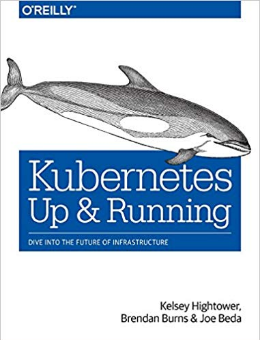
\includegraphics[height=20mm]{images/kubernetes-up-and-running.png}
       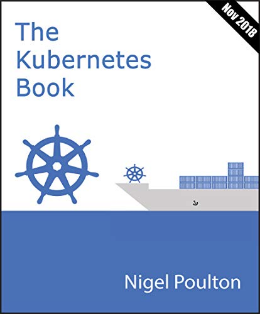
\includegraphics[height=20mm]{images/the-kubernetes-book.png}
       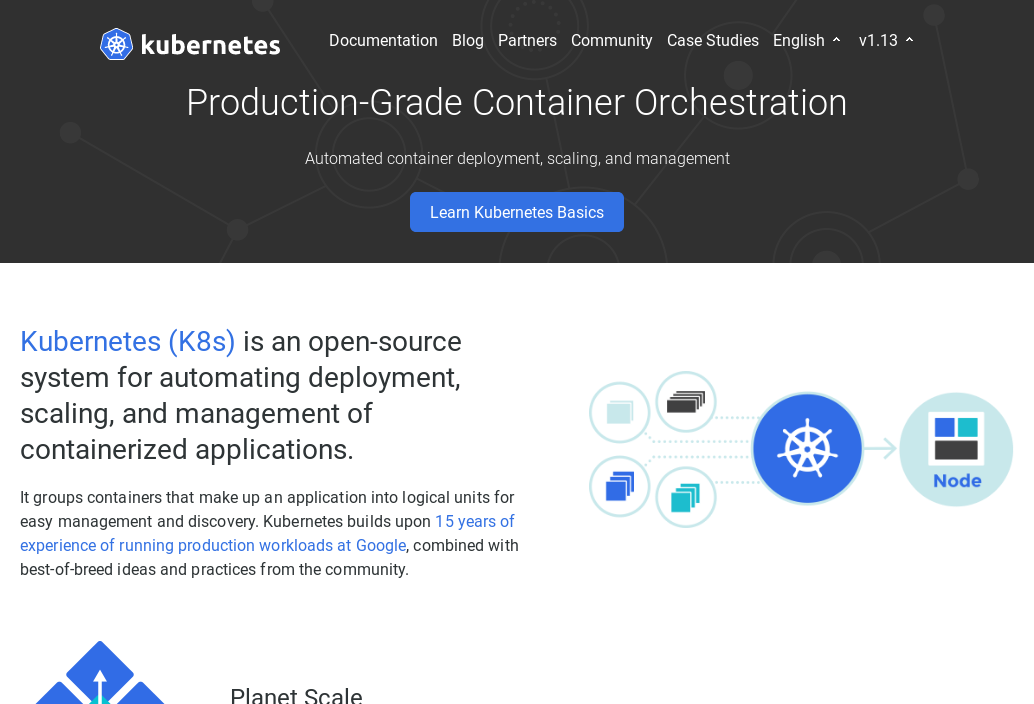
\includegraphics[height=20mm]{images/kubernetes-io.png}
    \end{itemize}
  \end{itemize}
\end{frame}

\begin{frame}
  \frametitle{Appendix}
  \begin{itemize}
      \item Slides: \url{https://bit.ly/k8s-the-hard-way-fossasia2019}
      \item Contact info: \texttt{masayukig on
        \href{https://freenode.net/}{Freenode},
        \href{https://github.com/masayukig}{GitHub},
        \href{https://twitter.com/masayukig}{Twitter},
        \href{https://www.linkedin.com/in/masayukig/}{LinkedIn}}
      \item Kubernetes The Hard Way: \url{https://github.com/kelseyhightower/kubernetes-the-hard-way}
  \end{itemize}
\end{frame}


\end{document}
